\documentclass{article}
% \usepackage{../../../lib/latex/draculatheme}
\usepackage{import}
\documentclass{article}
\usepackage[paper=letterpaper,margin=2cm]{geometry}
\usepackage[utf8]{inputenc}
\usepackage[russian]{babel}
\usepackage[]{graphicx}
\usepackage[usenames]{color}
\usepackage{colortbl}
\usepackage{geometry}
\usepackage{xcolor}
\usepackage{hyperref}
\usepackage{../../lib/latex/listings-rust}
\usepackage{fontspec}
\setmonofont{JetBrains Mono}[Contextuals=Alternate,Ligatures = TeX,]
\usepackage{listings}
\usepackage{keycommand}
\usepackage{caption}

\setmainfont[
  Ligatures=TeX,
  Extension=.otf,
  BoldFont=cmunbx,
  ItalicFont=cmunti,
  BoldItalicFont=cmunbi,
]{cmunrm}
\setsansfont[
  Ligatures=TeX,
  Extension=.otf,
  BoldFont=cmunsx,
  ItalicFont=cmunsi,
]{cmunss}

\geometry{
  a4paper,
  top=25mm,
  right=30mm,
  bottom=25mm,
  left=30mm
}

\hypersetup{
  colorlinks=true,
  linkcolor=blue!50!red,
  urlcolor=blue!70!black
}

\captionsetup[lstlisting]{
  font={tt},
}

% based on Atom One Light
\lstset{
  language=Java,
  frame=single,
  basicstyle=\ttfamily\color[HTML]{383a42},
  columns=fullflexible,
  breaklines=true,
  numbers=left,
  frame=tab,
  postbreak=\mbox{\textcolor{red}{$\hookrightarrow$}\space},
  extendedchars=false,
  showspaces=false,
  showstringspaces=false,
  identifierstyle=\ttfamily\color[HTML]{4078f2},
  commentstyle=\color[HTML]{a0a1a7},
  stringstyle=\color[HTML]{50a14f},
  keywordstyle=\color[HTML]{a626a4},
  numberstyle=\ttfamily\color[HTML]{2c91af},
  rulecolor=\color[HTML]{383a42}
}

\lstdefinelanguage{XML}
{
  morestring=[b]",
  morestring=[s]{>}{<},
  morecomment=[s]{<?}{?>},
}

\newcommand{\code}[1]{
  \lstset{title=#1}
  \lstinputlisting{#1}
}
\newkeycommand{\itmo}[variant=aboba, labn=aboba, discipline=aboba, group=aboba, student=aboba,teacher=aboba, year=2022]{
  \begin{titlepage}
    \begin{center}
      \section*{
        Федеральное государственное автономное образовательное учреждение\\ высшего образования\\
        «Национальный исследовательский университет ИТМО»\\
        Факультет Программной Инженерии и Компьютерной Техники \\
       }
      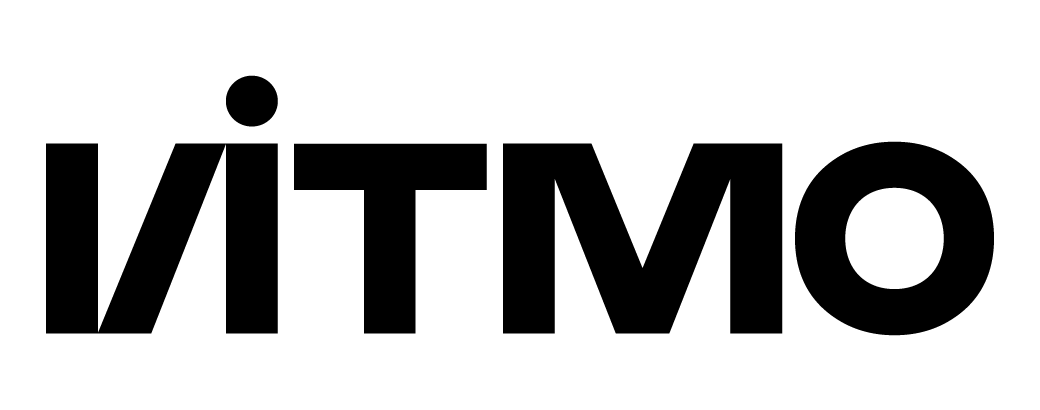
\includegraphics[scale=0.2]{../../lib/img/itmo.png}
    \end{center}

    \vspace{4cm}

    \begin{center}
      \large \textbf{Вариант \textnumero \commandkey{variant}}\\
      \textbf{Лабораторная работа \textnumero \commandkey{labn}}\\
      по дисциплине\\
      \textbf{\commandkey{discipline}}
    \end{center}

    \vspace*{\fill}

    \begin{flushright}
      Выполнил Студент группы \commandkey{group}\\
      \textbf{\commandkey{student}}\\
      Преподаватель: \\
      \textbf{\commandkey{teacher}}\\
    \end{flushright}

    \vspace{1cm}

    \begin{center}
      г. Санкт-Петербург\\
      \commandkey{year}г.
    \end{center}

    \thispagestyle{empty}
  \end{titlepage}
}



\begin{document}

\itmo[
  variant=74273.99,
  labn=6,
  discipline=Программирование,
  group=P3115,
  student=Владимир Мацюк,
  teacher=Кустарев Иван Павлович,
  year=2023,
  logo=../../../lib/img/itmo.png
]

\section*{Задание}

Разделить программу из лабораторной работы №5 на клиентский и серверный модули. Серверный модуль должен осуществлять выполнение команд по управлению коллекцией. Клиентский модуль должен в интерактивном режиме считывать команды, передавать их для выполнения на сервер и выводить результаты выполнения.

\section*{Необходимо выполнить следующие требования:}
\begin{itemize}
  \item Операции обработки объектов коллекции должны быть реализованы с помощью Stream API с использованием лямбда-выражений.
  \item Объекты между клиентом и сервером должны передаваться в сериализованном виде.
  \item Объекты в коллекции, передаваемой клиенту, должны быть отсортированы по умолчанию
  \item Клиент должен корректно обрабатывать временную недоступность сервера.
  \item Обмен данными между клиентом и сервером должен осуществляться по протоколу UDP
  \item Для обмена данными на сервере необходимо использовать датаграммы
  \item Для обмена данными на клиенте необходимо использовать сетевой канал
  \item Сетевые каналы должны использоваться в неблокирующем режиме.
\end{itemize}

\section*{Обязанности серверного приложения:}
\begin{itemize}
  \item Работа с файлом, хранящим коллекцию.
  \item Управление коллекцией объектов.
  \item Назначение автоматически генерируемых полей объектов в коллекции.
  \item Ожидание подключений и запросов от клиента.
  \item Обработка полученных запросов (команд).
  \item Сохранение коллекции в файл при завершении работы приложения.
  \item Сохранение коллекции в файл при исполнении специальной команды, доступной только серверу (клиент такую команду отправить не может).
\end{itemize}

\section*{Серверное приложение должно состоять из следующих модулей (реализованных в виде одного или нескольких классов):}
\begin{itemize}
  \item Модуль приёма подключений.
  \item Модуль чтения запроса.
  \item Модуль обработки полученных команд.
  \item Модуль отправки ответов клиенту.
\end{itemize}

Сервер должен работать в однопоточном режиме.

\section*{Обязанности клиентского приложения:}
\begin{itemize}
  \item Чтение команд из консоли.
  \item Валидация вводимых данных.
  \item Сериализация введённой команды и её аргументов.
  \item Отправка полученной команды и её аргументов на сервер.
  \item Обработка ответа от сервера (вывод результата исполнения команды в консоль).
  \item Команду save из клиентского приложения необходимо убрать.
  \item Команда exit завершает работу клиентского приложения.
\end{itemize}

Важно! Команды и их аргументы должны представлять из себя объекты классов. Недопустим обмен "простыми" строками. Так, для команды add или её аналога необходимо сформировать объект, содержащий тип команды и объект, который должен храниться в вашей коллекции.

\section*{Дополнительное задание:}
Реализовать логирование различных этапов работы сервера (начало работы, получение нового подключения, получение нового запроса, отправка ответа и т.п.) с помощью Log4J2

\section*{Отчёт по работе должен содержать:}

\begin{itemize}
  \item Текст задания.
  \item Диаграмма классов разработанной программы (как клиентского, так и серверного приложения).
  \item Исходный код программы.
  \item Выводы по работе.
\end{itemize}


\section*{Диаграмма классов}

\begin{center}
  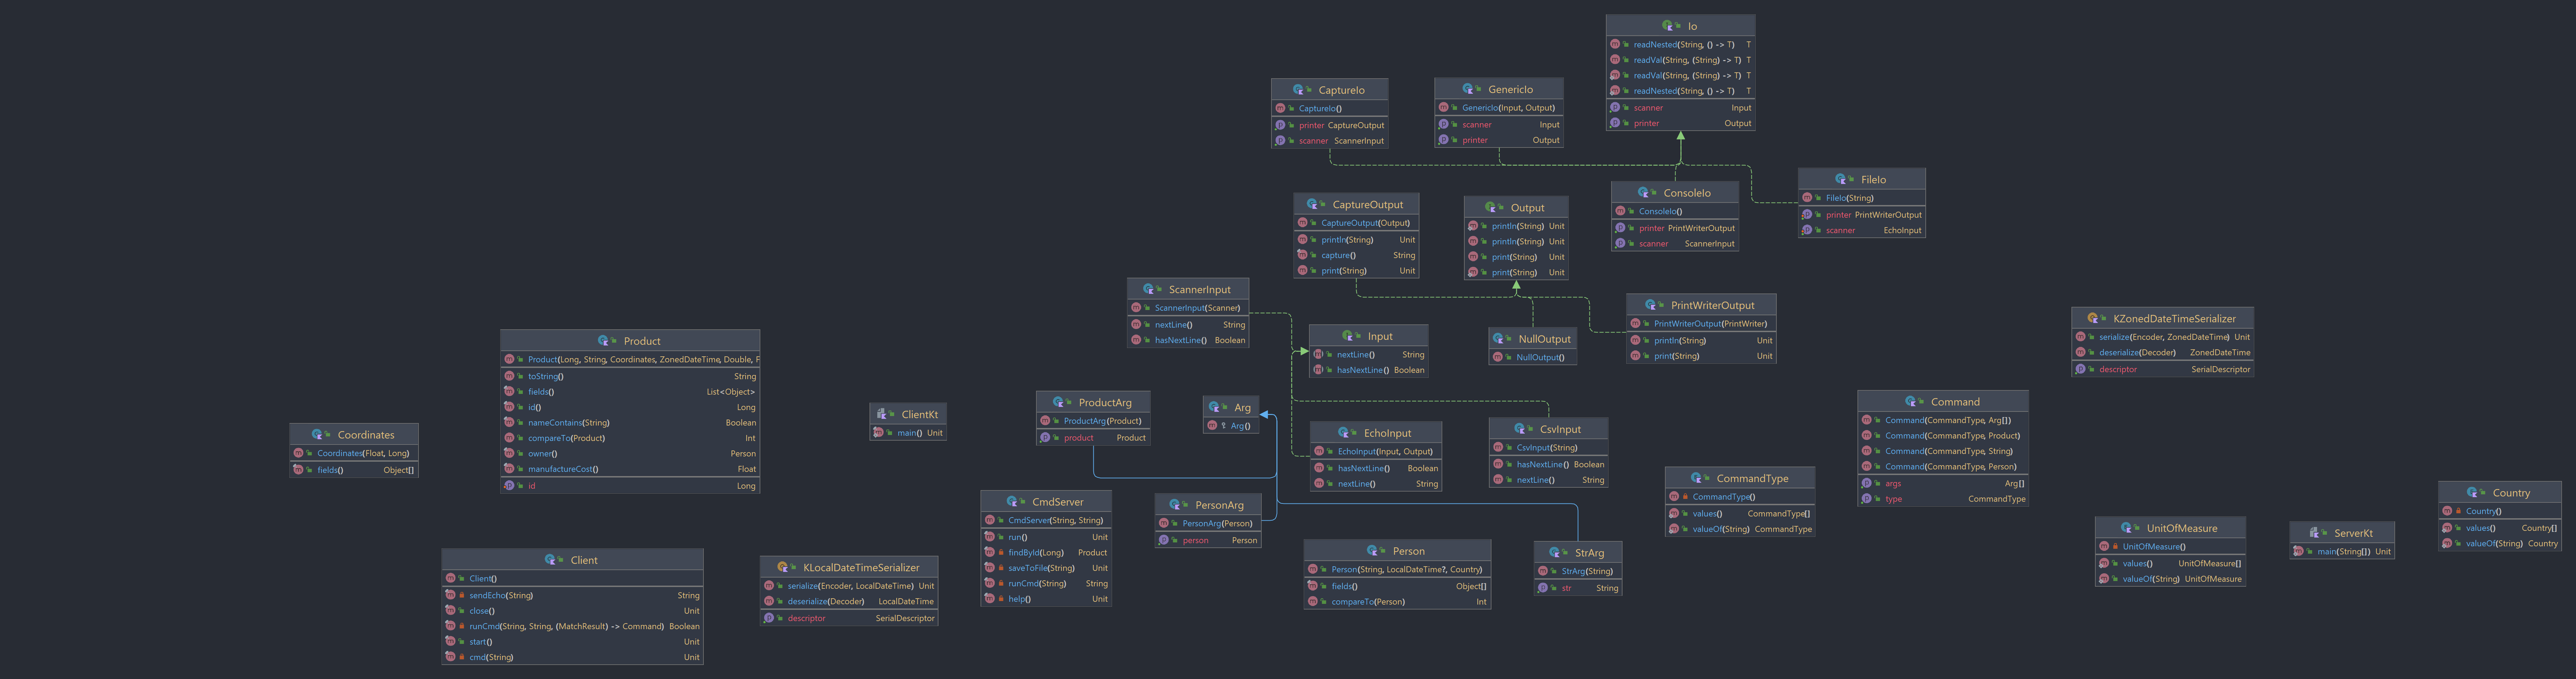
\includegraphics[scale=0.07]{diagram.png}
\end{center}

\section*{Исходный код}
\url{https://github.com/Wgmlgz/itmo2/tree/main/l6}

\section*{Вывод}
Во время выполнения работы я глубже ознакомился с ООП на языке java.
\end{document}
